\documentclass[slidestop,compress,mathserif]{beamer}
%\usepackage[bars]{beamerthemetree} % Beamer theme v 2.2
%\usetheme{Antibes}
\usetheme{Copenhagen}
%\usetheme{Dresden}
%\usetheme{JuanLesPins}
%\usetheme{Boadilla}
%\usetheme{Rochester} %sobrio
% Beamer theme v 3.0
%\usecolortheme{lily}
%\usecolortheme{albatross}
%\usecolortheme{seahorse}
%\usecolortheme{beetle}
%\usecolortheme{crane}
%\usecolortheme{dolphin}
%\usecolortheme{dove}
%\usecolortheme{fly}
%\usecolortheme{lily}
%\usecolortheme{orchid}
%\usecolortheme{rose}
%\usecolortheme{seagull}
\usecolortheme{whale}

%\usepackage{bbding}
\usepackage{pifont}
%\usepackage{fourier-orns}

\setbeamertemplate{navigation symbols}{}
\setbeamertemplate{footline}
{
\leavevmode
\hbox{
\begin{beamercolorbox}
[wd=.5\paperwidth,ht=2.5ex,dp=1.125ex,leftskip=.3cm plus1fill,rightskip=.3cm]
{author in head/foot}
\usebeamerfont{author in head/foot}\insertauthor
\end{beamercolorbox}%
\begin{beamercolorbox}[wd=.5\paperwidth,ht=2.5ex,dp=1.125ex,leftskip=.3cm,rightskip=.3cm plus1fill]
{title in head/foot}%
\usebeamerfont{title in head/foot}\insertshortinstitute
\end{beamercolorbox}}%
  \vskip0pt%
}

%\beamertemplateshadingbackground{blue!20}{white!40}
%\setbeamercolor{title}{fg=red!80!black,bg=red!20!white}
%\setbeamercolor{navigation symbols dimmed}{fg=red!80!black}
%\setbeamercolor{navigation symbols}{fg=red!80!black}

%COLORES DEL TITULO
%\setbeamercolor*{palette tertiary}{fg=white,bg=structure.black!60!green}
%\setbeamercolor*{palette secondary}{fg=white,bg=structure.black!50!green}
%\setbeamercolor*{palette primary}{use=structure,fg=white,bg=structure.black!40!green}
%\setbeamercolor{itemize item}{fg=red}

% Beamer color theme
\usepackage [utf8]{inputenc}

% General data
\title[Master Thesis and experiences]
{Free Software Master Thesis and experiences}
%\subtitle {Solamente si hay subtítulo}
\author[Autores abreviados]{Antonio Arias Losada}
\institute{Free Software Master - 2011/2012}


\begin{document}

\begin{frame}
% Cover slide
\titlepage
\begin{center}

\includegraphics[height=1cm]{images/igalia.png}
\hspace{10mm}

\includegraphics[height=1cm]{images/urjc.png}
\end{center}
\end{frame}

\begin{frame}
\frametitle{Table of contents}

\tableofcontents[hideallsubsections]
\end{frame}


\section{Introduction}
%\1ction{Master Thesis: Crosscompilation of the open source web browser engine WebKitGTK+ for the ARMv7 processors family}
\begin{frame}
\frametitle{Introduction}

\end{frame}

\section{Master Thesis}
\subsection{Objectives}
\begin{frame}
\frametitle{Objectives}

The main objective is building a Linux based image for ARM processors architecture with a WebKit2 web browser.
The achieve the main goal, the work was divided the following subobjectives:

\vspace{5mm}

\begin{enumerate}
\item<1-> Compile WebKit.
\item<2-> Prepare Yocto environment.
\item<3-> Create a Yocto image for ARM and run it with QEMU.
\item<4-> Create a Yocto image for ARM with WebKit.
\end{enumerate}

\end{frame}

\subsection{Motivation}
\begin{frame}
\frametitle{Motivation}

This work is motivated basically by two key points:
\pause

\vspace{10mm}
\begin{center}

\includegraphics[height=1.5cm]{images/HTML5-logo.png}
\hspace{10mm}
\pause

\includegraphics[height=0.8cm]{images/ARM-logo.png}
\end{center}

\end{frame}

\subsection{Results}
\begin{frame}
\frametitle{Results}

\begin{block}{Task \#1}<1->
WebKit2 GTK+ compiled for AMD64 architecture.
\end{block}

\begin{block}{Task \#2}<2->
Yocto environment prepared.
\end{block}

\begin{block}{Task \#3}<3->
Generated and ran an ARM image.
\end{block}

\begin{alertblock}{Task \#4}<4->
Compile WebKit2 GTK+ for ARM architecture.
\end{alertblock}

\end{frame}

\section{Experiences}
\subsection{MFS Open sessions 2011}
\begin{frame}
\frametitle{MFS Open sessions 2011}
Introductory talk about Open Source Hardware in the open sessions of the Free Software Master 2011 edition, collaborating with Xulio Coira.

\begin{center}

\includegraphics[height=5cm]{images/ohw-logo.png}
\end{center}

\end{frame}

\subsection{OSHWDEM 2012}
\begin{frame}
\frametitle{OSHWDEM 2012}
OSHWDEM 2012 celebrated in A Coru\~na, on 17/11/2012.

\begin{center}
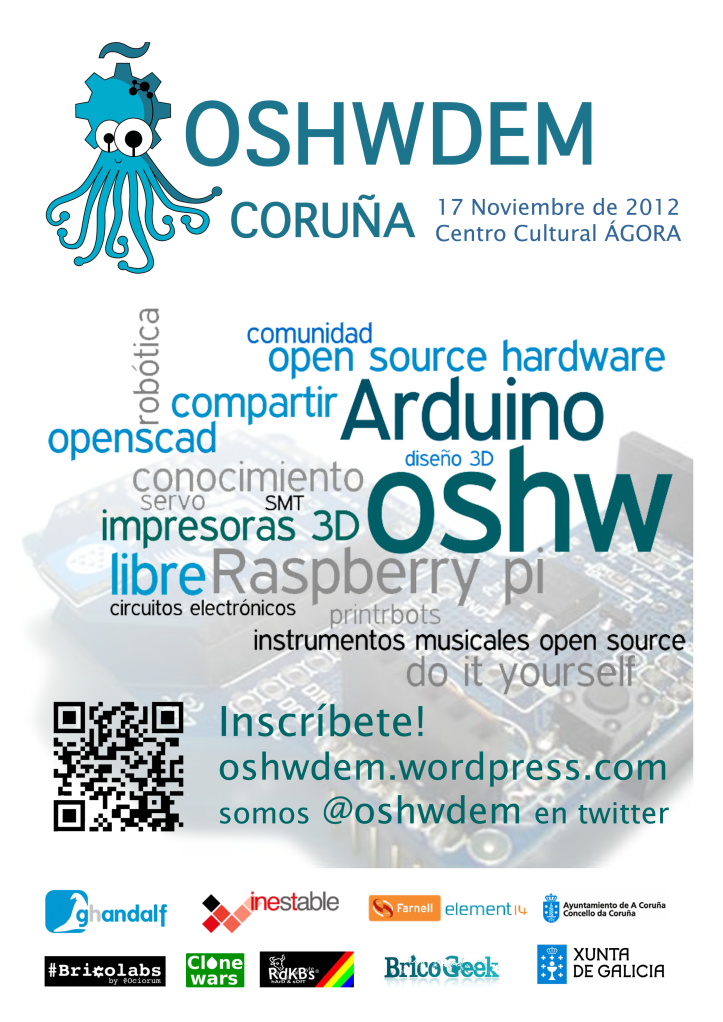
\includegraphics[height=6.5cm]{images/cartel-oshwdem5-300.png}
\end{center}

\end{frame}

\end{document}